\documentclass{report}
\usepackage[utf8]{inputenc}
\usepackage{graphicx}
\usepackage{amsmath}
\usepackage{mathtools}
\usepackage{physics}
\usepackage{float}
\usepackage{amsfonts}
\usepackage{hyperref}


\title{The Heat Equation}
\author{Aryan Garg}
\date{February 2022}

\newcommand{\heatequation}[0]{\frac{\partial T}{\partial t}(x,t) = \alpha \frac{\partial^2 T}{\partial x^2}(x,t)}
\newcommand\scalemath[2]{\scalebox{#1}{\mbox{\ensuremath{\displaystyle #2}}}}

\begin{document}

\maketitle

\begin{abstract}
    In this paper I will be outlining the process towards solving the heat equation, starting from the
    basic knowledge of ODE's. This paper will be looking at this problem from a
    high level and will not get too much into the details on how one might go about solving PDE's. 
    Instead, this paper is meant to give an introduction to the reader on what it means to read and solve a PDE.
\end{abstract}


\chapter{Introduction To The Heat Equation}
\section{What Is A Differential Equation?}

A differential equation essentially relates a function to its own derivatives or "rate of change." We can 
see this for example in the following ordinary differential equation
\[\dv{x}{t} = 3x + 4\]
This equation states that the function $x(t)$ rate of change is equal to 3 times its current value $+ 4$
If we were to solve this equation, we would get
\[x(t) = \frac{e^{3t+c_1}}{3}-\frac{4}{3} \]

This same intuition can be carried on for partial differential equations
For example, if we say that
\[ \pdv{F}{x} = \pdv{F}{y} \]

This statement essentially states that however our function $F(x,y)$ changes with respect to $x$ 
will be equal to how our function $F(x,y)$ changes with respect to $y$.
One possible solution to this equation could be:
\[F(x,y) = x+y\]
\[ \pdv{F}{x} = 1 = \pdv{F}{y} \]

\section{The Heat Equation}
So what exactly is our heat equation? 
\[ \heatequation \]
Where $T(x,t)$ is the temperature equation that gives the temperature at each point $x$ at 
the time $t$ of an object (which in our case will be a rod)

\begin{figure}[h]
    \centering
    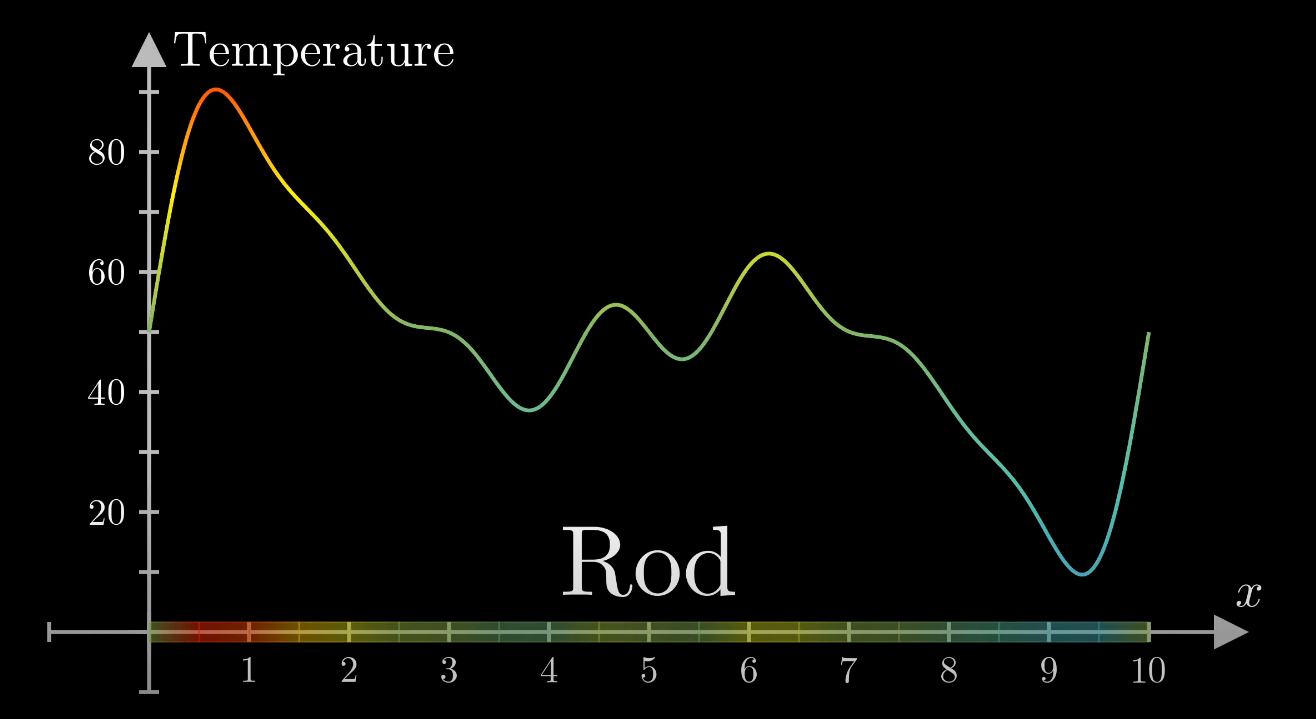
\includegraphics[width=0.8\textwidth]{images/temperature_distribution_on_rod.PNG}
    \caption{Example temperature distribution of $T(x,0)$ of our rod}
\end{figure}

So what is our heat equation stating explicitly? 
Well it states that for a small step in time, $\partial t$, the change in temperature ($\partial T$)
will be equal to some constant $\alpha$ multiplied by the second derivative of how the 
temperature changes on the rod ($\pdv[2]{T}{x}$), or in other words the "curvature" of the
the temperature distribution at each point x.

This all seems quite abstract, let's see if we can get some more intuition on how this equation was formed.

\section{Intuition Behind The Heat Equation}

Well, one of the most obvious things about our heat equation is that it should make sure 
that the colder parts of our rod heat up, and the warmer parts of our rod cool down. 

Another intuitive thought about our heat equation is that the speed at which each point cools down or warms up
should be related to that point's neighbors. For example, if the temperature of the points around 
a point $x$ is a lot less than the temperature at $x$, then the temperature at $x$ should change
more rapidly compared to if the neighboring points around $x$ were about its same temperature. 

Now that we understand the main intuitions behind the heat equation, we just need a way to quantify this.
To determine how much the neighboring points around a point x change related to itself, we can use 
the rate of rate of change, or the second derivative. 

A way to think about this is that everywhere the temperature distribution curves, we would expect that 
"curve" to flatten out over time. If it curves downward, we would expect the temperature to fall. If it curves upward, we expect the temperature to rise. And, however, "fast" our function curves around our point $x$
will determine the speed at which the temperature will rise or fall. If the points around $x$ curve at a high rate, we would expect our  temperature to change at a high rate, and if it curves at a small rate we would expect our temperature to change only a little bit.

\begin{figure}[h]
    \centering
    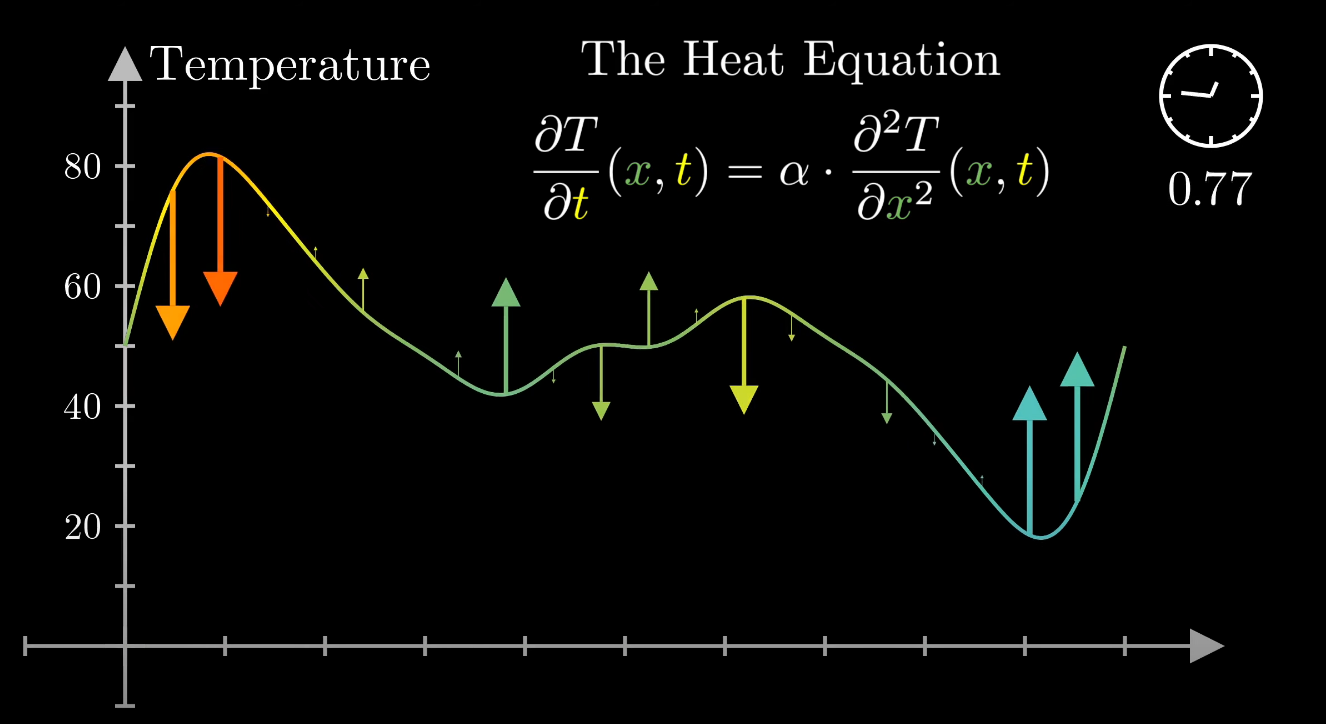
\includegraphics[width=0.8\textwidth]{images/intutition_behind_heat_equation.png}
    \caption{Example of how our temperature distribution might change}
\end{figure}

So in conclusion, we can now say with confidence that: 
\[ \frac{\partial T}{\partial t} \propto \frac{\partial^2 T}{\partial x^2} \]

And adding some constant $\alpha$:
\[ \frac{\partial T}{\partial t} = \alpha \frac{\partial^2 T}{\partial x^2} \]

\chapter{Solving The Heat Equation In Idealized Situations}

\section{Solving the Heat Equation with $\sin(x)$}

So now how would we ever even start with trying to solve the monster that is the heat equation?
Well for a start, one thing we can try to do is look at an idealized situation. For example,
with a little playing around we might ask ourselves what will happen if we were to make
our initial temperature distribution model a sine wave. That is:

$$T(x,0) = \sin(x)$$

While this is obviously unrealistic, if we take the second partial derivative we can see that it might actually
take us somewhere closer to solving the heat equation.

\[ \pdv{T}{x} = \cos(x)\]
\[ \pdv[2]{T}{x} = -\sin(x) = -T\]

Plugging this all back into our heat equation:
\[ \heatequation \]
\[ \pdv{T}{t} = -\alpha T \]

This form looks kind of familiar... Let's see what happens if we change the $\partial$ to a $d$

\[ \dv{T}{t} = -\alpha T\]
\[ \frac{1}{T} \, dT=-\alpha \, dt \]
\[ \int\frac{1}{T} \, dT=\int-\alpha \, dt \]
\[ \ln(T) = -\alpha t \]
\[ T = e^{-\alpha t} \]

So now we have two equations
\[ T = \sin(x) \]
\[ T = e^{-\alpha t} \]
After some playing around, we might decide to try and combine the two equations to try and find $T(x,t)$

\begin{equation} \label{solution_with_sin}
    T(x,t) = \sin(x)e^{-\alpha t} 
\end{equation}

and if we were to check if this equation is a solution to our heat equation:
\[ \heatequation \]
\[ T(x,t) = \sin(x)e^{-\alpha t} \]
\begin{minipage}{0.45\textwidth}
  \begin{align*}
      \pdv{T}{t} = -\alpha \sin(x)e^{-\alpha t}
    \end{align*}
\end{minipage}
\begin{minipage}{0.45\textwidth}
    \begin{align*}
        \pdv{T}{x} &= \cos(x)e^{-\alpha t} \\
        \pdv[2]{T}{x} &= -\sin(x)e^{-\alpha t} 
    \end{align*}
\end{minipage}

\[ -\alpha \sin(x)e^{-\alpha t} = \alpha (-\sin(x)e^{-\alpha t} ) \]

Wow! So we see that $T(x,t) = \sin(x)e^{-\alpha t}$ is a solution to our heat equation!

\pagebreak

If we look at a graph of $T(x,t) = \sin(x)e^{-\alpha t}$, the function also does seem to look like
how we would expect a temperature function to look

\begin{figure}[H]
    \centering
    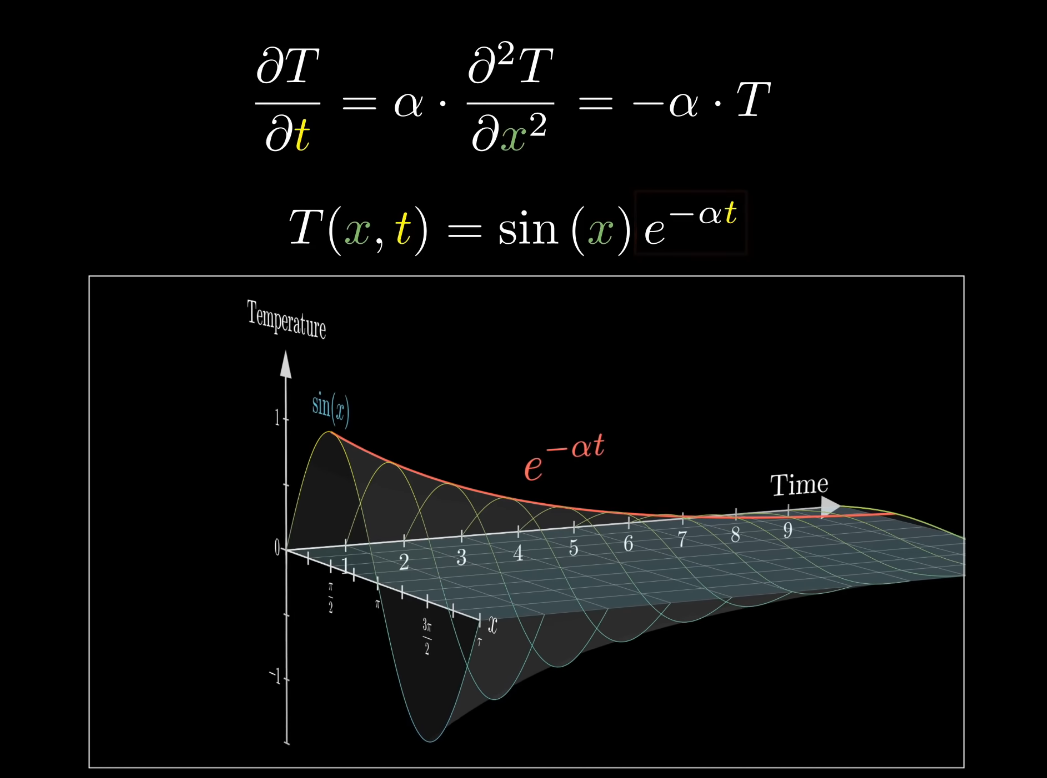
\includegraphics[width=0.7\textwidth]{images/sinx_temperature_function.png}
    \caption{A 3D model of $T(x,t) = \sin(x)e^{-\alpha t}$ }
\end{figure}

\begin{figure}[H]
    \centering
    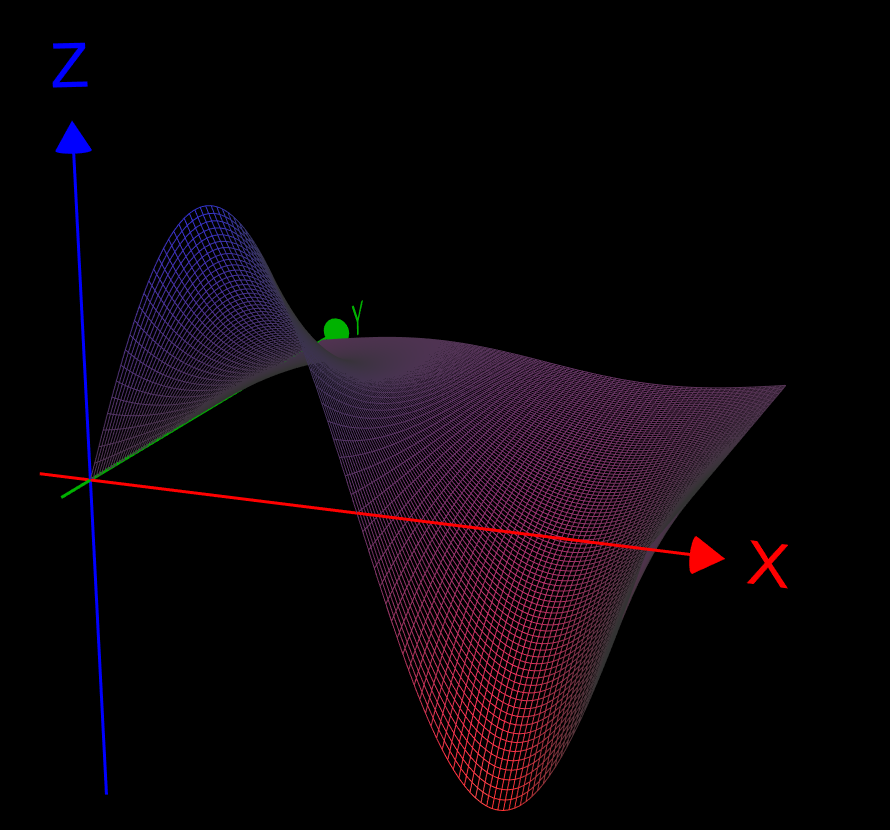
\includegraphics[width=0.7\textwidth]{images/sinx_temperature_function_2.png}
    \caption{Another view of $T(x,t) = \sin(x)e^{-\alpha t}$ (axes are: $z = T$, $y = t$) }
\end{figure}

While this function at first look does seem to match our intuition on how the temperature
function might look, at further exploration, you might see that the two ends of our rod never change in temperate, which
does not seem that realistic. 

At even more exploration you might realize that even $T(x,t) = x$ also seems to be a valid solution
to our heat equation

\begin{figure}[H]
    \centering
    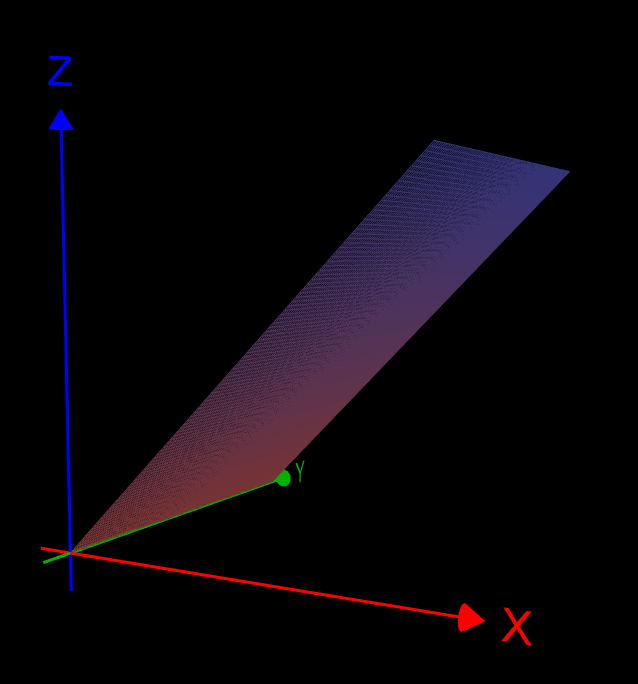
\includegraphics[width=0.7\textwidth]{images/x_no_boundary_function.png}
    \caption{The graph of $T(x,t) = x$ (axes are: $z = T$, $y = t$) }
\end{figure}

This function is obviously wrong, as the temperature never even changes at any point, but it IS a valid solution to our
heat equation. It feels we are missing something, some type of limiting factor.

\section{Boundary Conditions}

Our current heat equation seems to be missing some type of limiting factor, or in other words a boundary condition.

There are different types of boundary conditions that we can apply to our heat equation, but in this paper, we will
explore the boundary condition if our bar had perfectly insulated boundaries (or in other terms, no heat escapes or enters 
into the boundaries of our rod). 

One place where we can search for a limiting factor is two ends of our rod, one at $x=0$ and the other at $x=L$,
Where $L$ is the length of our rod.
In our current solution for the heat equation, we can see that  $T(0,t) = 0$ and $T(L,t) = 0$ for all $t$, which 
does not seem realistic. One thing we could imagine is that instead of the two ends of the rod always being at 0\textdegree, we can match the temperature of the two ends with their neighbors. To quantify this, we can say: 
\[ \frac{\partial T}{\partial x}(0,t) = \frac{\partial T}{\partial x}(L,t) = 0 \]

Now to try and find a solution to our new pair of equations $\heatequation$ and the above boundary condition, let's see if we can make any modifications to the original solution we found:

\[T(x,0) = \sin(x) \]
\[ T(x,t) = \sin(x)e^{-\alpha t} \]

What if instead of $\sin(x)$, we used $\cos(x)$? Then $\pdv{T}{x}|_{x=0} = 0$. We need to adapt 
$\cos(x)$ so that $\pdv{T}{x}|_{x=L} = 0$ is also true. We can do this by modifying the period of 
$\cos(x)$ to:
\[\cos(\frac{\pi}{L}x)\]
Which we can further generalize to 
\[\cos(\frac{\pi n}{L}x)\]
And if we were to call $\omega = \frac{\pi n}{L}$, we can finally say:
\[T(x,0) = \cos(\omega x) \]
Since we are changing the inner value of $\cos$ though, our $\pdv[2]{T}{x}$ will be different so we need to recalculate 
$T(x,t)$
\[ \pdv{T}{x} = -\omega\sin(\omega x) \]
\[ \pdv[2]{T}{x} = -\omega^2\cos(\omega x) = -\omega^2T\]
Plugging this all back in
\[\heatequation\]
\[\pdv{T}{t} = -\alpha\omega^2T \]
\[ T = e^{-\alpha\omega^2t} \]

Now if we combine the two as we did back in Equation\ref{solution_with_sin}, we can finally say:


\begin{equation} \label{soln_with_cos}
     T(x,t) = \cos(\omega x)e^{-\alpha\omega^2t} 
\end{equation}
where
\[ \omega = \frac{\pi n}{L} \qquad n \in \mathbb{Z} \qquad L = \textrm{Length of rod} \]

And if we were to check if this function followed our heat equation $\heatequation$ and our boundary
conditions $\frac{\partial T}{\partial x}(0,t) = \frac{\partial T}{\partial x}(L,t) = 0 $ we will find that it is a valid solution. 

The diagram of this new solution to our heat equation also looks a lot more realistic to how a temperature distribution
might look. 

\begin{figure}[H]
    \centering
    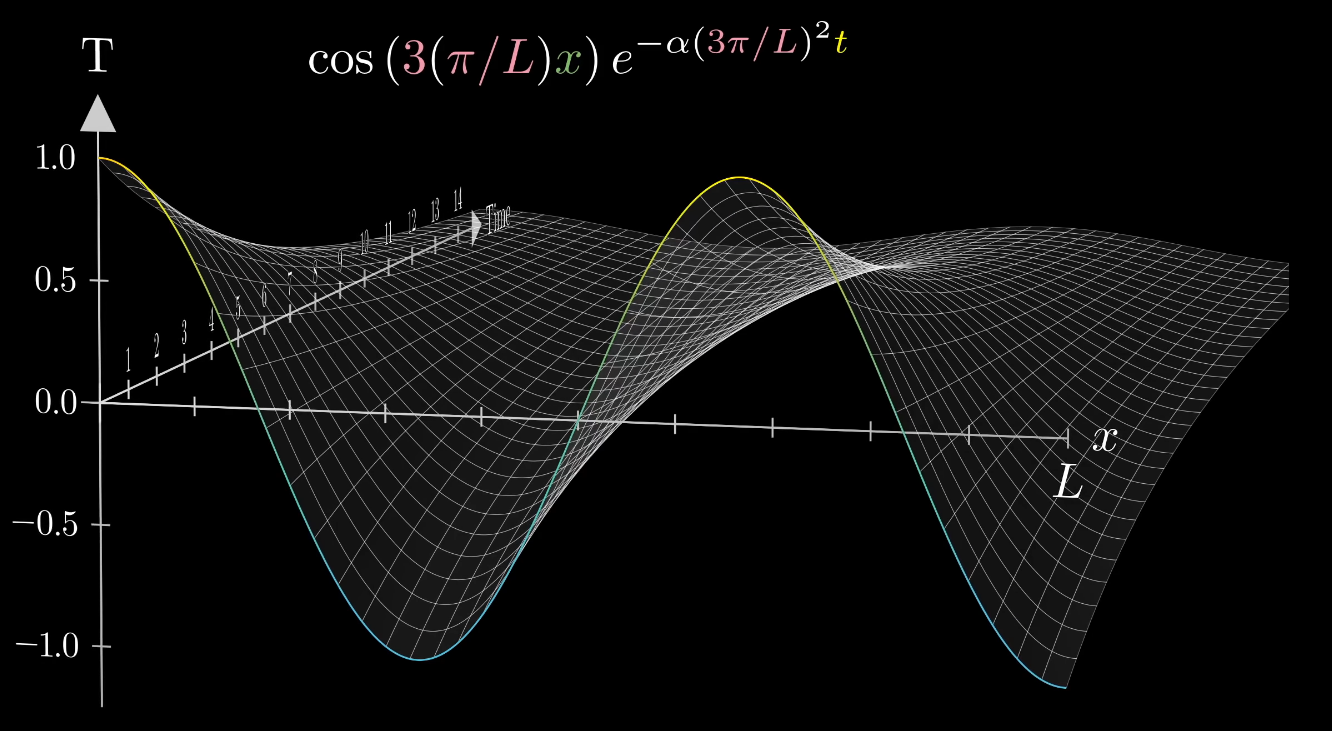
\includegraphics[width=0.9\textwidth]{images/cosx_temperature_function.png}
    \caption{The graph of $T(x,t) = \cos(\omega x)e^{-\alpha\omega^2t}$ where $n = 3$}
\end{figure}

\begin{figure}[H]
    \centering
    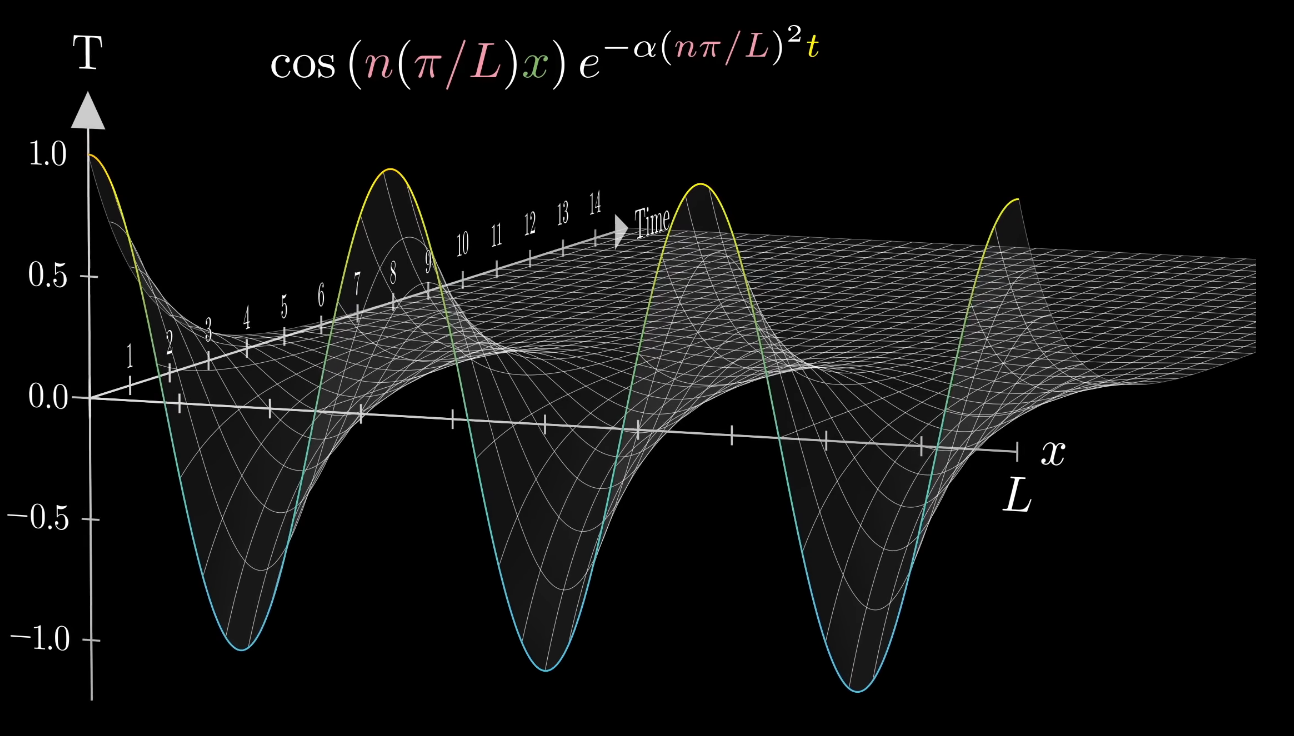
\includegraphics[width=0.9\textwidth]{images/cosx_temperature_function_2.png}
    \caption{And remember, since $n \in \mathbb{Z}$ we actually found an infinite set of solutions to our heat equation }
\end{figure}


\section{Linearity of The Heat Equation}
Great, so we finally found a solution to the heat equation. In fact, we found an infinite set of solutions to our heat equation, but the problem is that all of these solutions are cosine waves. Is there any way we can generalize this out of just cosine waves? 

Well one property we can exploit to help us is the superposition principle. It turns out that the solution for a temperature curve made up of two (or more) cosine waves is equal to the two solutions of each curve separately added together. 

That is if we set our initial conditions to:
\[ T(x,0) = \cos( \frac{\pi}{L}x ) + \cos( \frac{2\pi}{L}x )\]
\[ \omega_1 = \frac{\pi}{L} \qquad \omega_2 = \frac{2\pi}{L}\]
\[ T(x,0) = \cos( \omega_1x ) + \cos( \omega_2x )\]

We can easily find the solutions to each of these separately using 
the equation we found back in \ref{soln_with_cos}:

\[ \heatequation \]
\[ T(x,t) = \cos(\omega x)e^{-\alpha\omega^2t}  \]

\begin{minipage}{0.45\textwidth}
  \begin{align*}
      T_1(x,0) &= \cos( \omega_1x ) \\
      T_1(x,t) &= \cos(\omega_1 x)e^{-\alpha\omega_1^2t} 
    \end{align*}
\end{minipage}
\begin{minipage}{0.45\textwidth}
    \begin{align*}
        T_2(x,0) &= \cos( \omega_2x ) \\
        T_2(x,t) &= \cos(\omega_2 x)e^{-\alpha\omega_2^2t} 
    \end{align*}
\end{minipage}

\vspace{10pt}

With the superposition principle we can say: 

\[T(x,t) = T_1(x,t) + T_2(x,t) \]
\begin{equation} \label{two_cos_heat_eq_soln}
     T(x,t) = \cos(\omega_1 x)e^{-\alpha\omega_1^2t} + \cos(\omega_2x)e^{-\alpha\omega_2^2t}
\end{equation}

Great, so we can find a solution to a set of cosine waves added together, but what does such a graph of two waves even look like?

\begin{figure}[H]
    \centering
    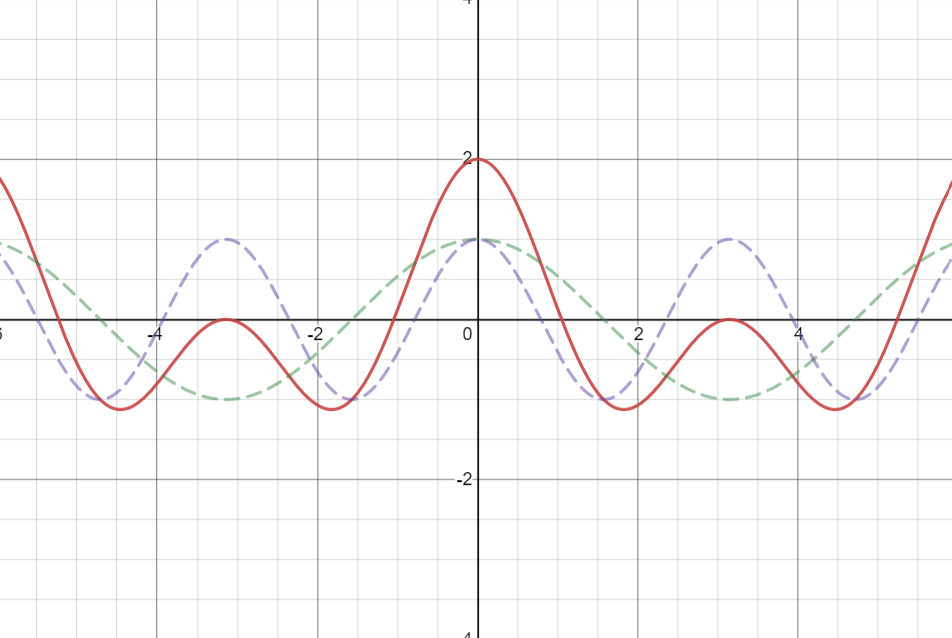
\includegraphics[width=0.75\textwidth]{images/graph_of_two_cos.png}
    \caption{Graph of $\cos(x) + \cos(2x)$ in red}
\end{figure}

We can see that at certain points the two waves add together and 
create a large displacement from $x=0$, but at other points, they cancel out.

Below we can see the graph of the temperature equation of this weird combination of waves.

\begin{figure}[H]
    \centering
    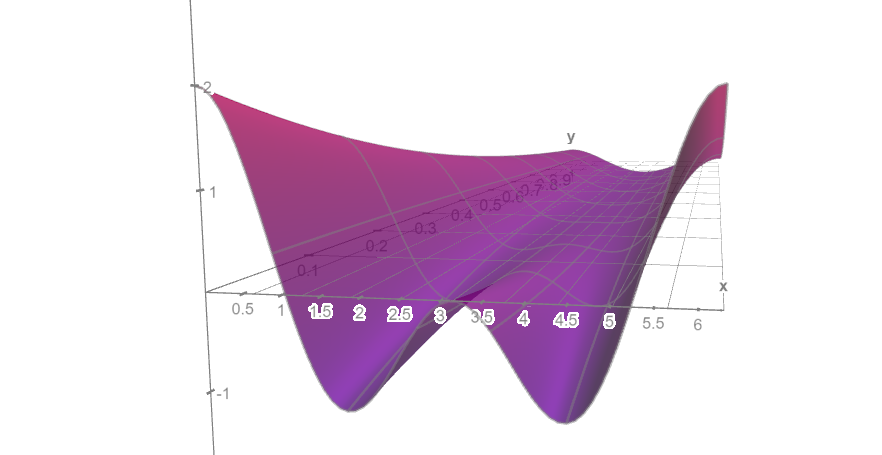
\includegraphics[width=0.75\textwidth]{images/graph_of_two_cos_heat_equation.png}
    \caption{Sample heat equation for $T(x,0) = \cos(x) + \cos(2x)$}
\end{figure}

\chapter{Fourier Series}
\section{Deriving the Fourier Series}

Great, so we can find a solution to our heat equation with cosine waves with varying periods 
and summations of cosine waves with varying periods, but how does this help us with trying to model 
how heat flows in a more realistic temperature distribution? 

For example, if we had two rods, one of them at some low temperature and another we heated up to some
high temperature, and we connected the two together. What would the temperature distribution look like? 

\begin{figure}[H]
    \label{two_rods_touching_figure}
    \centering
    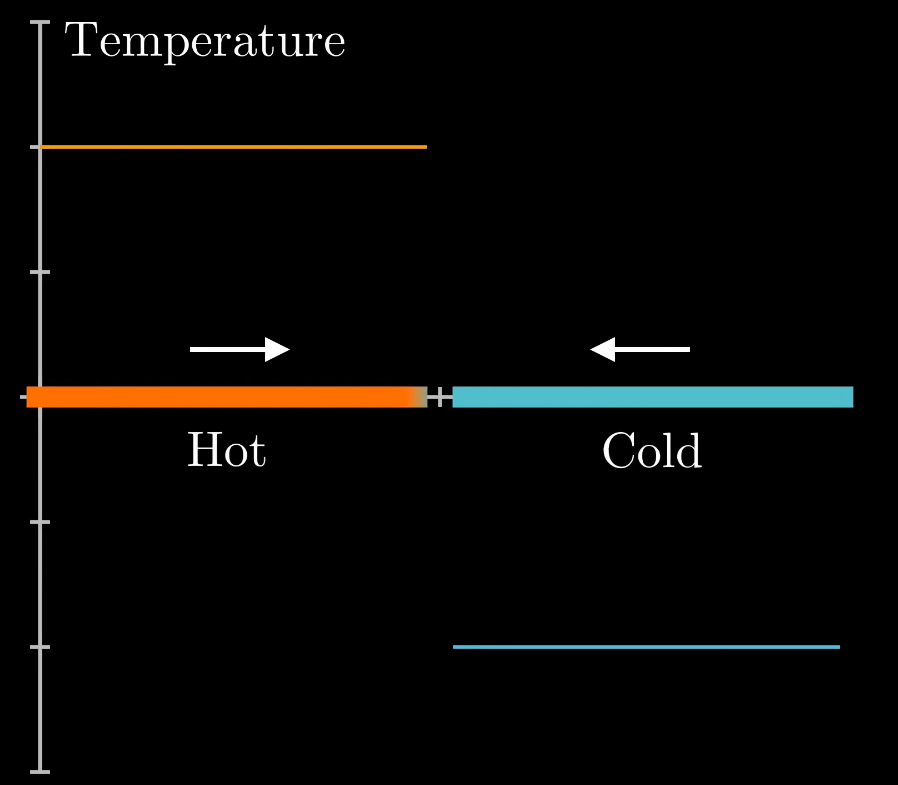
\includegraphics[width=0.75\textwidth]{images/sample_two_rods_distribution.png}
    \caption{Sample $(T(x,0)$ graph for two rods of differing heat touching}
\end{figure}

In the early 1800s, Joseph Fourier was phased with a similar dilemma when trying to solve the heat equation.
One insight that he thought of was that what if we could represent an equation as a summation of $\cos$ and $\sin$ waves?

That is: what if we represented our function $f(x)$ as:
\[ f(x)= c_0 + \sum_{n=1}^{\infty} a_n\cos(nx) + \sum_{n=1}^{\infty} b_n\sin(nx) \]
Now all we would need to do is solve for all the constants $a_n$ and $b_n$ for all $n$. To do this, one property we can exploit is the orthogonality of the 
trigonometric functions, which states:

\[ \int_{-\pi}^{\pi} (\sin(mx) \cos(nx)) \, dx = 0 \quad \textrm{for} \quad n \in \mathbb{Z} \quad m \in \mathbb{Z}  \]
\[ \int_{-\pi}^{\pi} (\sin(mx) \sin(nx)) \, dx = 0 \quad \textrm{for} \quad n \in \mathbb{Z} \quad m \in \mathbb{Z} \quad n \neq m  \]
\[ \int_{-\pi}^{\pi} (\cos(mx) \cos(nx)) \, dx = 0 \quad \textrm{for} \quad n \in \mathbb{Z} \quad m \in \mathbb{Z} \quad n \neq m  \]

I will not be proving the above properties in this paper, but they can easily be derived using basic trigonometric identities and is left as an exercise to the reader. 

For now lets ignore our initial constant $c_0$ and try and manipulate our above function of $f(x)$ into solving for $a_n$ 
\[ f(x)= \sum_{n=1}^{\infty} a_n\cos(nx) + \sum_{n=1}^{\infty} b_n\sin(nx) \]
\[ \cos(mx)(f(x))= \cos(mx) \left( \sum_{n=1}^{\infty} a_n\cos(nx) + \sum_{n=1}^{\infty} b_n\sin(nx) \right) \]
\[ \int_{-\pi}^{\pi} \cos(mx)f(x) \, dx = \int_{-\pi}^{\pi} \cos(mx) \left( \sum_{n=1}^{\infty} a_n\cos(nx) + \sum_{n=1}^{\infty} b_n\sin(nx) \right) \, dx \]
By our orthogonality properties above, we can state that all the terms in $\sum_{n=1}^{\infty} b_n\sin(nx)$ will end up as 0,
and all the terms in $\sum_{n=1}^{\infty} a_n\cos(nx)$ will go to 0 except for the term $n = m$
\[ \int_{-\pi}^{\pi} \cos(mx)f(x) \, dx = \int_{-\pi}^{\pi} \cos(mx) (a_m\cos(mx)) \, dx \]
\[ \int_{-\pi}^{\pi} \cos(mx)f(x) \, dx = \int_{-\pi}^{\pi} a_m \cos^2(mx) \, dx \]
\[ \int_{-\pi}^{\pi} \cos(mx)f(x) \, dx = a_m \int_{-\pi}^{\pi} \cos^2(mx) \, dx \]
Changing some variables around to look like the standard form
\[ \int_{-\pi}^{\pi} \cos(nx)f(x) \, dx = a_n \int_{-\pi}^{\pi} \cos^2(nx) \, dx \]
\[ \int_{-\pi}^{\pi} \cos^2(nx) \, dx = \pi \quad  \textrm{for} \quad n \in \mathbb{Z} \]
\[ \int_{-\pi}^{\pi} \cos(nx)f(x) \, dx = a_n \pi \]
\[ a_n = \frac{1}{\pi} \int_{-\pi}^{\pi} \cos(nx)f(x) \, dx \]
Using a similar derivation, we can find $b_n$ to be:
\[ b_n = \frac{1}{\pi} \int_{-\pi}^{\pi} \sin(nx)f(x) \, dx \]

To find $c_0$ what we can do is multiple both sides by $\cos(0x) = 1$ and integrate both sides.
Because of the orthogonality property we discussed earlier, all the $\cos$ and $\sin$ terms will go to 0.
\[ \int_{-\pi}^{\pi} \cos(0x)(f(x)) \, dx = 
\int_{-\pi}^{\pi} \cos(0x) \left( c_0 + \sum_{n=1}^{\infty} a_n\cos(nx) + \sum_{n=1}^{\infty} b_n\sin(nx) \right) \, dx \]
\[\int_{-\pi}^{\pi} f(x) \, dx = c_0 \int_{-\pi}^{\pi} \, dx\]
\[ 2\pi c_0 = \int_{-\pi}^{\pi} f(x) \, dx \]
\[ c_0 = \frac{1}{2\pi}\int_{-\pi}^{\pi} f(x) \, dx \]
Now we have a formula for $c_0$ as well. Analytically, the formula also seems right as it states that $c_0$ equals
the average value of $f(x)$. So where you want to "start" the summation of (or the amount you want to translate up of)
the different $\sin$ and $\cos$ waves will be equal to the average value of $f(x)$.

Also just to add on some syntactic sugar, we are going to state that: 
\[\frac{a_0}{2} = \frac{1}{2\pi}\int_{-\pi}^{\pi} f(x) \, dx = c_0\]
\[c_0 = \frac{a_0}{2} \]


So now going back to our original equation, we finally have a formula for $a_0$, $b_0$ and $c_0$
\[ f(x)= c_0 + \sum_{n=1}^{\infty} a_n\cos(nx) + \sum_{n=1}^{\infty} b_n\sin(nx) \]

\[ \scalemath{0.825}{
f(x)= \frac{a_0}{2} + \frac{1}{\pi} \sum_{n=1}^{\infty} \left( \left( \int_{-\pi}^{\pi} \cos(nx)f(x) \, dx \right) \cos(nx) \right)
+ \frac{1}{\pi} \sum_{n=1}^{\infty} \left( \left( \int_{-\pi}^{\pi} \sin(nx)f(x) \, dx \right) \sin(nx) \right) }
\]

So we finally finished deriving the Fourier Series Formula, at least for $\cos(nx)$ and $\sin(nx)$ with periods of of $2\pi$
The more generalized Fourier Series formula for adding up $\cos$ and $\sin$ functions with periods of $P$ is:

\[f(x) = \frac{a_{0}}{2}+\sum_{n=1}^{\infty}\left(a_{n} \cos \left(\frac{2 \pi}{P} n x\right)+b_{n} \sin \left(\frac{2 \pi}{P} n x\right)\right) \]

\[\begin{aligned}
a_{n} &=\frac{2}{P} \int_{P} f(x) \cdot \cos \left(\frac{2 \pi}{P} n x\right) d x \\ 
b_{n} &=\frac{2}{P} \int_{P} f(x) \cdot \sin \left(\frac{2 \pi}{P} n x\right) d x
\end{aligned} \]

\pagebreak

\section{Solving The Heat Equation For Two Rods Touching }
Referring back to Figure \ref{two_rods_touching_figure}, let us try to assemble a formula for the temperature distribution function
$T(x,0)$. Also, let us try to make this formula have an average value of $0$ to eliminate our $c_0$ term and make the function
an even function as this will eliminate the $\sin$ terms.

\[ T(x,0) =
    \begin{dcases}
        1 & 0\leq x \leq 0.5 \\
        0 & x = 0.5 \\
        -1 & 0.5 \leq x \leq 1 \\
    \end{dcases}
\]

We can see that our formula for $T(x,0)$ represents a step function. 

Since we want this step function to be even let us define the periodic function $f(x)$ of which we will expand with the Fourier Series as:

\[ f(x) =
    \begin{dcases}
        1 & -0.5 + 2n\leq x \leq 0.5 + 2n \\
        0 & x = 0.5 + 2n \\
        -1 & 0.5 + 2n \leq x \leq 1.5 + 2n \\
    \end{dcases}
\]

\begin{figure}[H]
    \centering
    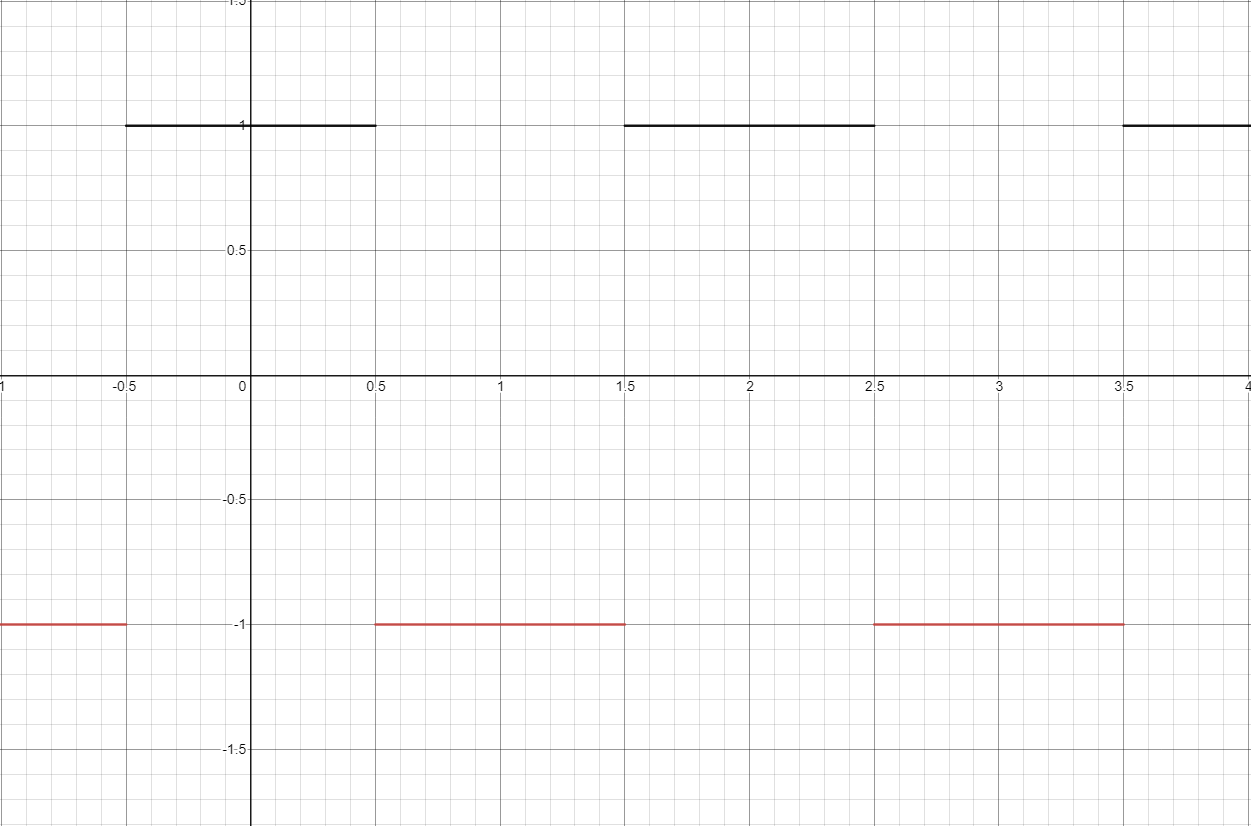
\includegraphics[width=0.8\textwidth]{images/step_function_graph.png}
    \caption{Graph of f(x)}
\end{figure}


Now let's find the Fourier Series for $f(x)$

\[f(x) = \frac{a_{0}}{2}+\sum_{n=1}^{\infty}\left(a_{n} \cos \left(\frac{2 \pi}{P} n x\right)+b_{n} \sin \left(\frac{2 \pi}{P} n x\right)\right) \]

\[\begin{aligned}
a_{n} &=\frac{2}{P} \int_{P} f(x) \cdot \cos \left(\frac{2 \pi}{P} n x\right) d x \\ 
b_{n} &=\frac{2}{P} \int_{P} f(x) \cdot \sin \left(\frac{2 \pi}{P} n x\right) d x
\end{aligned} \]

\[P = [-0.5,1.5] = 2 \]
\[ \frac{a_0}{2} = \int_{-0.5}^{1.5} f(x) \, dx = \int_{-0.5}^{0.5} \, dx  - \int_{0.5}^{1.5} \, dx = 0\] 

\[f(x) = \sum_{n=1}^{\infty}\left(a_{n} \cos \left(\pi n x\right)+b_{n} \sin \left(\pi n x\right)\right) \]
\[
a_{n} = \int_{-0.5}^{1.5} f(x) \cdot \cos \left(\pi n x\right) \, dx
= \int_{-0.5}^{0.5} \cos \left(\pi n x\right) \, dx - \int_{0.5}^{1.5} \cos \left(\pi n x\right) \, dx
\]
\[
b_{n} = \int_{-0.5}^{1.5} f(x) \cdot \sin \left(\pi n x\right) \, dx
= \int_{-0.5}^{0.5} \sin \left(\pi n x\right) \, dx - \int_{0.5}^{1.5} \sin \left(\pi n x\right) \, dx
\]

As I said above, since $f(x)$ is an even function all the $\sin$ terms ( $b_n$ ) will = 0. We can quickly show this:
\[b_n = \int_{-0.5}^{0.5} \sin \left(\pi n x\right) \, dx - \int_{0.5}^{1.5} \sin \left(\pi n x\right)\]
\[= -\frac{1}{\pi n}\ \left( \cos(\pi n x) |_{-0.5}^{0.5} - \cos(\pi n x) |_{0.5}^{1.5}  \right) \]
\[= -\frac{1}{\pi n}\ \left( \cos( \frac{\pi}{2}n )  - \cos( -\frac{\pi}{2}n ) - \cos( \frac{3\pi}{2}n ) + \cos( \frac{\pi}{2}n ) \right) = 0\]
\[b_n = 0 \]

So now all we need to do is calculate $a_n$, which will give us all the coefficients for the $\cos$ waves which make up $f(x)$, which we can
easily use to finally connect it all back into solving our heat equation. 

% https://www.desmos.com/calculator/ub1vizzc2f

\[
a_{n} = \int_{-0.5}^{0.5} \cos \left(\pi n x\right) \, dx - \int_{0.5}^{1.5} \cos \left(\pi n x\right) \, dx
\]
\[= \frac{1}{\pi n}\left( \sin(\pi n x) |_{-0.5}^{0.5} - \sin(\pi n x) |_{0.5}^{1.5}  \right)  \]
\[= \frac{1}{\pi n}\ \left( \sin( \frac{\pi}{2}n )  - \sin( -\frac{\pi}{2}n ) - \sin( \frac{3\pi}{2}n ) + \sin( \frac{\pi}{2}n ) \right)\]
\[= \frac{1}{\pi n}\ \left( 3\sin( \frac{\pi}{2}n )  - \sin( \frac{3\pi}{2}n ) \right)\]

Now that we have a formula for $a_n$, let us see what our Fourier expansion looks like
\[f(x) = \sum_{n=1}^{\infty} a_{n} \cos \left(\pi n x\right) \]
\[f(x) = \frac{4}{\pi}\cos(\pi x) - \frac{4}{3 \pi}\cos(3 \pi x) + \frac{4}{5\pi}\cos(5\pi x) - \dots \]
\[f(x) = \frac{4}{\pi}\sum_{n=1}^{\infty}\frac{\left(-1\right)^{n+1}}{2n-1}\cos\left(\left(2n-1\right)\pi x\right) \]

So we found a solution for $f(x)$ in terms of $\cos$ curves. What does this Fourier expansion actually look like?
Well we can see at first it does not look very accurate but it starts to quickly converge onto $f(x)$\footnote{You might notice at the discontinuities of the graph that the Fourier Series does not converge onto $f(x)$. This is called Gibbs Phenomenon.}

\begin{figure}[H]
    \centering
    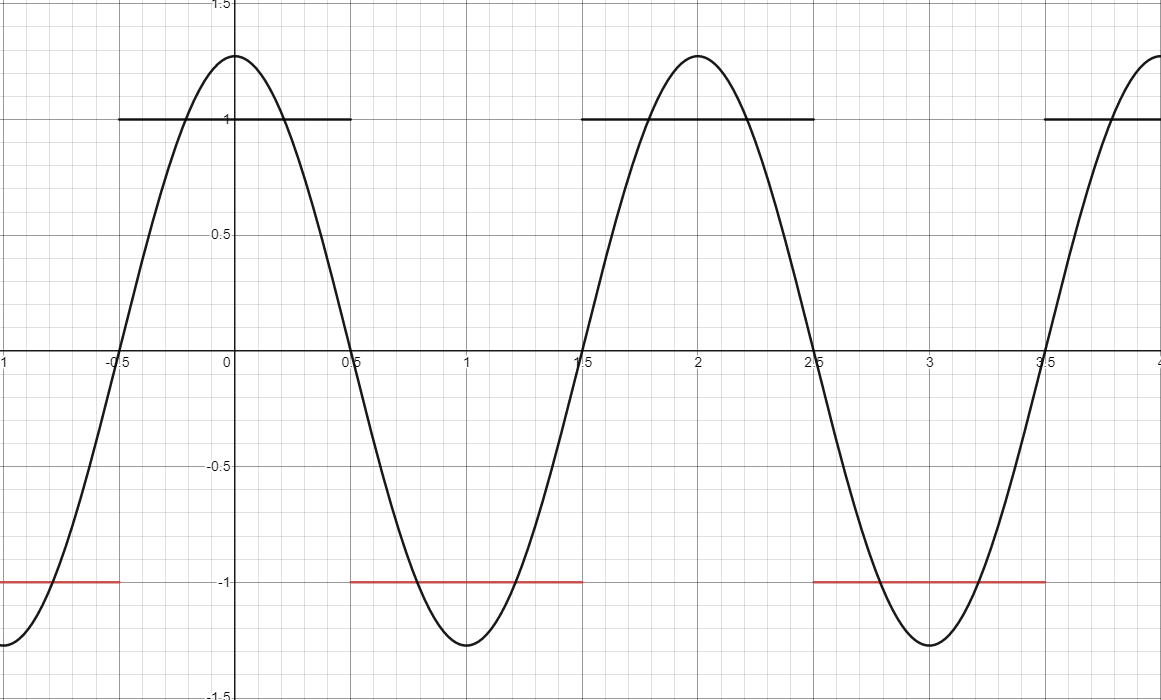
\includegraphics[width=0.9\textwidth]{images/fourier_series/fourier_1.png}
    \caption{Fourier Series of $f(x)$ with $N=1$}
\end{figure}

\begin{figure}[H]
    \centering
    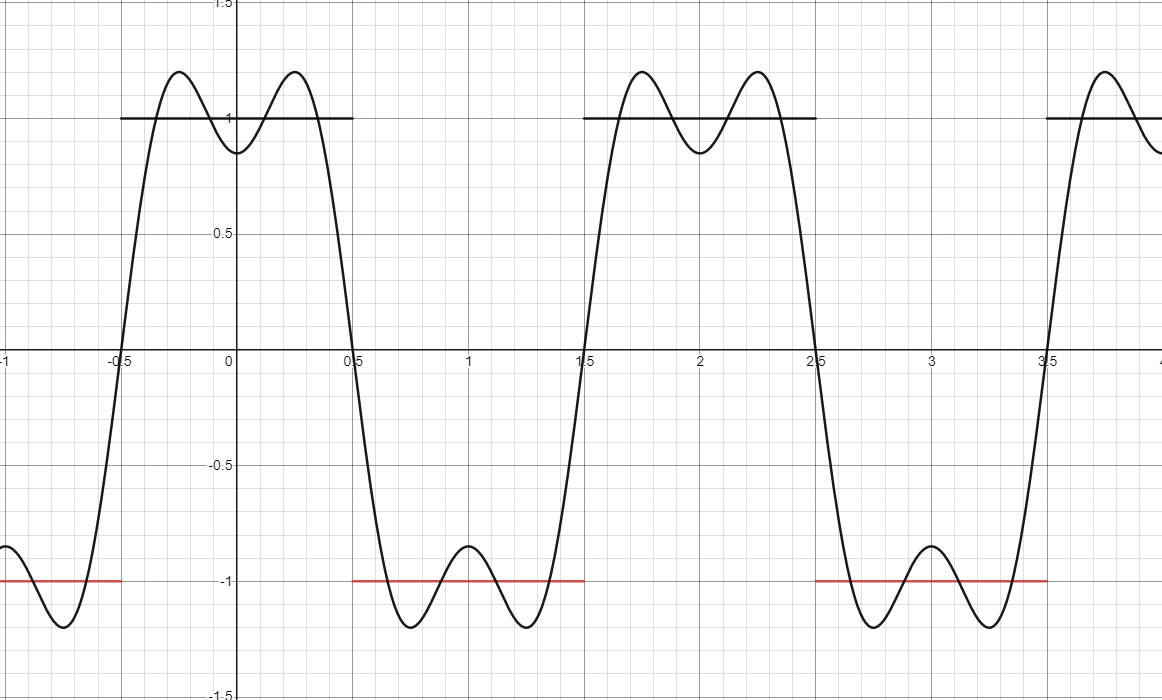
\includegraphics[width=0.9\textwidth]{images/fourier_series/fourier_2.png}
    \caption{Fourier Series of $f(x)$ with $N=2$}
\end{figure}

\begin{figure}[H]
    \centering
    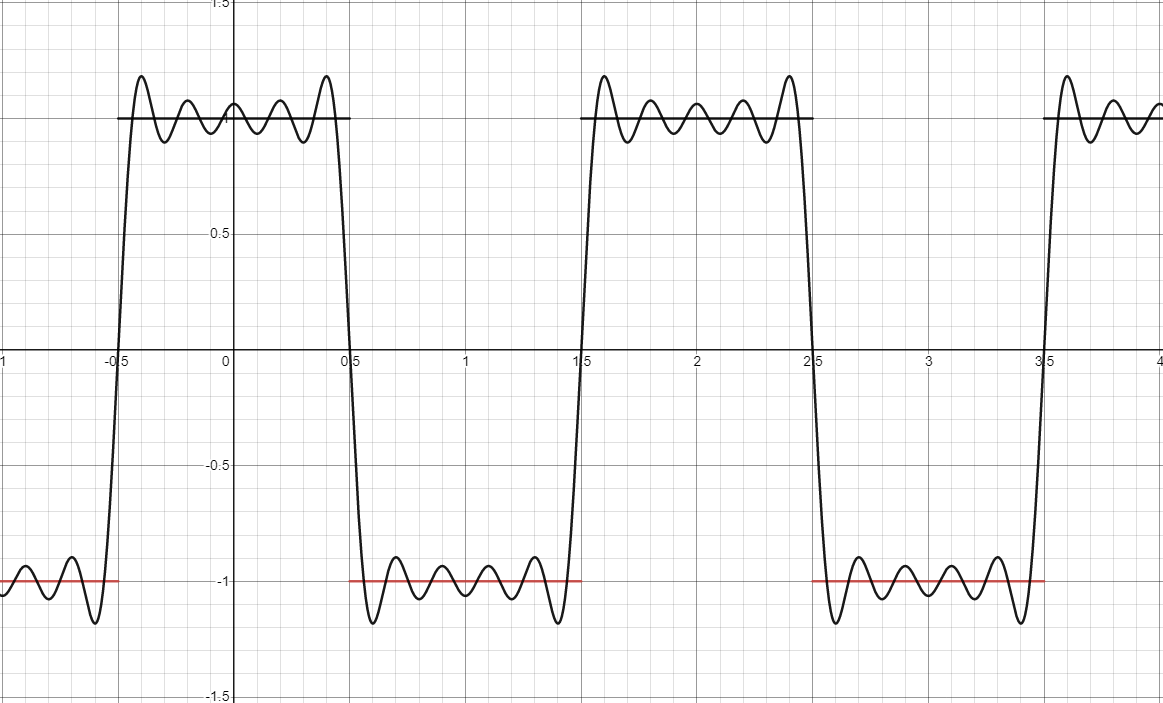
\includegraphics[width=0.9\textwidth]{images/fourier_series/fourier_5.png}
    \caption{Fourier Series of $f(x)$ with $N=5$}
\end{figure}

\begin{figure}[H]
    \centering
    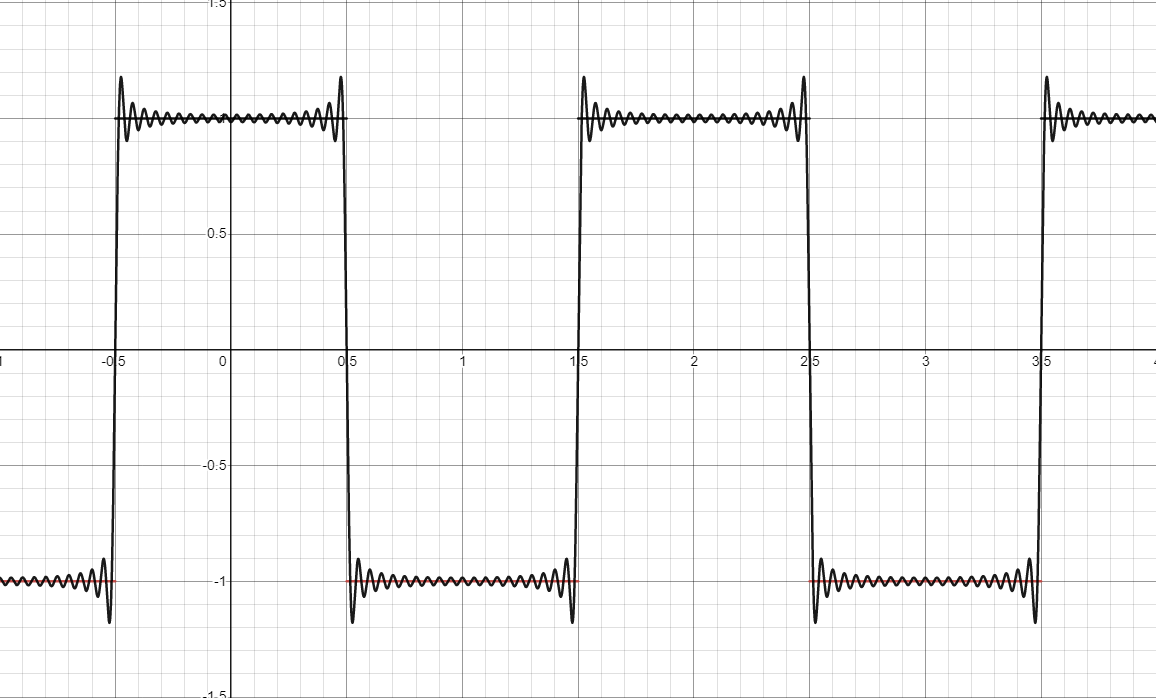
\includegraphics[width=0.9\textwidth]{images/fourier_series/fourier_20.png}
    \caption{Fourier Series of $f(x)$ with $N=20$}
\end{figure}

\begin{figure}[H]
    \centering
    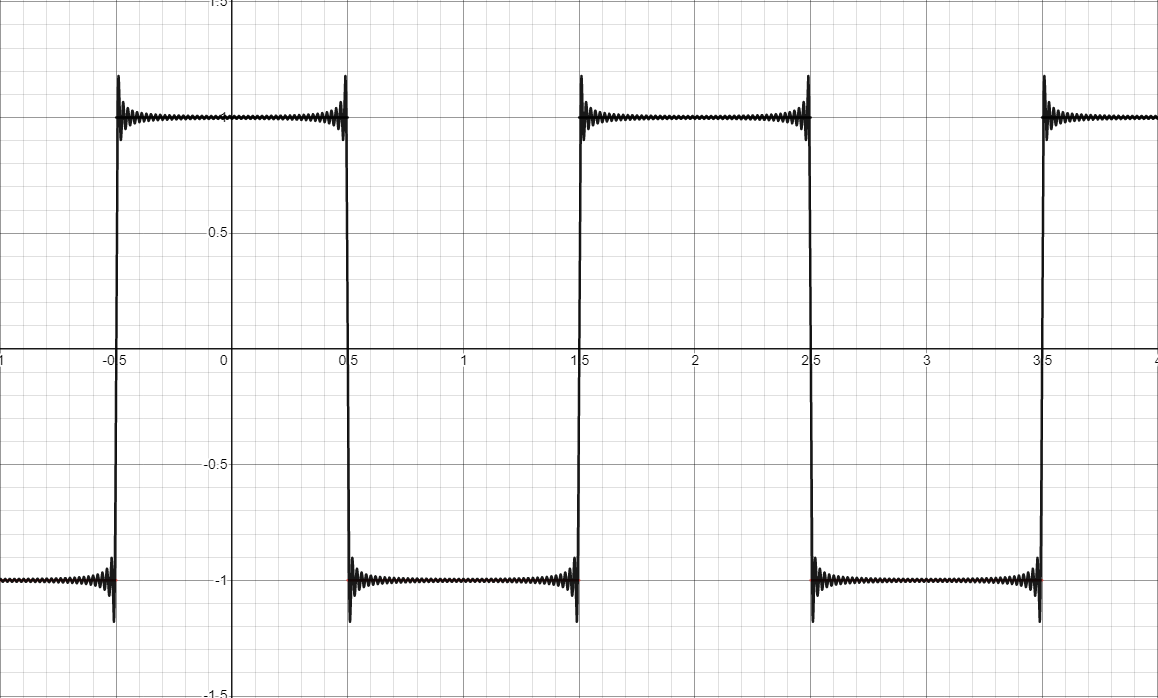
\includegraphics[width=0.8\textwidth]{images/fourier_series/fourier_50.png}
    \caption{Fourier Series of $f(x)$ with $N=50$}
\end{figure}

You can play around with these graphs more at \url{https://www.desmos.com/calculator/kwfjdrw1gv}

Finally, lets solve our heat equation $T(x,t)$, by going back to our solution to the heat equation:

\[ \heatequation \]
\[T(x,0) = \cos(\omega x) \]
\[T(x,t) = \cos(\omega x)e^{-\alpha\omega^2t} \quad \textrm{where} \quad \omega = \pi n\]

Now lets connect this back to the Fourier Series expansion of $T(x,0)$
\[ T(x,0) =
    \begin{dcases}
        1 & 0\leq x \leq 0.5 \\
        0 & x = 0.5 \\
        -1 & 0.5 \leq x \leq 1 \\
    \end{dcases}
\]
\[T(x,0) = \frac{4}{\pi}\sum_{n=1}^{\infty}\frac{\left(-1\right)^{n+1}}{2n-1}\cos\left(\left(2n-1\right)\pi x\right) \quad 0\leq x \leq 1 \]
\[\omega = (2n - 1)\pi \]
\[T(x,0) = 4\sum_{n=1}^{\infty}\frac{\left(-1\right)^{n+1}}{\omega}\cos\left(\omega x\right) \quad 0\leq x \leq 1 \]
\[T(x,t) = 4\sum_{n=1}^{\infty}\frac{\left(-1\right)^{n+1}}{\omega}\cos\left(\omega x\right)e^{-\alpha\omega^2t} \quad 0\leq x \leq 1 \]
% 4 ((e^(-π^2 y) cos(π x))/π - (e^(-9 π^2 y) cos(3 π x))/(3 π) + (e^(-25 π^2 y) cos(5 π x))/(5 π) - (e^(-49 π^2 y) cos(7 π x))/(7 π) + (e^(-81 π^2 y) cos(9 π x))/(9 π))

Here is what this graph looks like:

\begin{figure}[H]
    \centering
    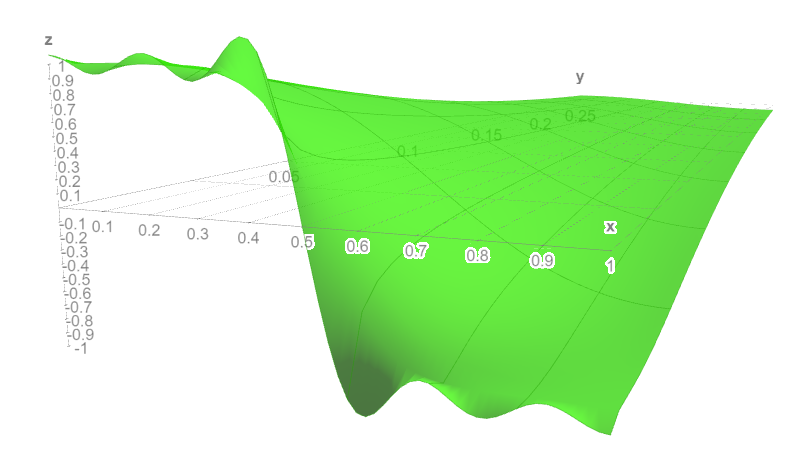
\includegraphics[width=0.9\textwidth]{images/two_rods_heat_equation_soln.png}
    \caption{Estimate graph (N=5) for $T(x,t)$, \quad  $y = t$}
\end{figure}

You can play around with this graph at \url{https://www.math3d.org/d9mHKfYHf}
You can also see a simulation of the heat equation at \url{https://www.desmos.com/calculator/rscofnudyv}

\chapter{Conclusion}
Finally, we were able to find a solution to the heat equation for pretty much any equation. 

This paper started off with the basics of differential equations and then introduced the idea of how to read partial differential equations. With that, we were then able to introduce the heat equation:
\[ \heatequation \]
and were able to derive every component of the heat equation.

We next moved on to solving a PDE. We started off with a specialized situation with:
\[ T(x,0) = \sin(x) \]
and we were able to find the solution to be
\[ T(x,t) = \sin(x)e^{-\alpha t}  \]

We then realized that we needed to get more specific with our PDE, and got introduced to the idea of boundary conditions.
We analyzed our boundary conditions to be: 
\[ \frac{\partial T}{\partial x}(0,t) = \frac{\partial T}{\partial x}(L,t) = 0 \]
And found a new set of solutions:
\[T(x,0) = \cos(\omega x) \]
\[ T(x,t) = \cos(\omega x)e^{-\alpha\omega^2t}  \]

We were able to further realize that we could incorporate the superposition principle into our solution and easily find the heat equation to multiple $\cos$ waves added together.

We were able to exploit this property using the Fourier Series, which states:
\[ f(x)= c_0 + \sum_{n=1}^{\infty} a_n\cos(nx) + \sum_{n=1}^{\infty} b_n\sin(nx) \]
We were able to find the Fourier series for 2 rods touching to be: 
\[ T(x,0) =
    \begin{dcases}
        1 & 0\leq x \leq 0.5 \\
        0 & x = 0.5 \\
        -1 & 0.5 \leq x \leq 1 \\
    \end{dcases}
\]
\[T(x,0) = 4\sum_{n=1}^{\infty}\frac{\left(-1\right)^{n+1}}{\omega}\cos\left(\omega x\right) \quad 0\leq x \leq 1 \]

and then using our previous heat equation solutions, we were able to find the heat equation solution to $T(x,t)$, and finally a strategy on how to find the heat equation for a more generalized situation.

\[T(x,t) = 4\sum_{n=1}^{\infty}\frac{\left(-1\right)^{n+1}}{\omega}\cos\left(\omega x\right)e^{-\alpha\omega^2t} \quad 0\leq x \leq 1 \]

We learned a lot about differential equations and PDE, equations that really rule and dictate our universe and everything that moves around in it ranging from quantum mechanics to fluid dynamics. 

We got to explore PDE's with the heat equation, a very important equation in the field of thermodynamics and a good first step into the vast world of PDE's. 

And arguable one of the most important things we learned in this paper was the Fourier Series, a very elegant piece of math that notoriously shows up everywhere, ranging from electrical engineering, acoustics, economics, and more! 

\begin{thebibliography}{5}
 \bibitem{3b1bRef} [3Blue1Brown's Video Series on Differential Equations] \url{https://www.youtube.com/playlist?list=PLZHQObOWTQDNPOjrT6KVlfJuKtYTftqH6}
 \bibitem{kahnRef} [Kahn Academy's Lessons on the Fourier Series] \url{https://www.khanacademy.org/science/electrical-engineering/ee-signals\#ee-fourier-series}
 \bibitem{paulsRef} [Paul's Online Notes: Solving The Heat Equation] \url{https://tutorial.math.lamar.edu/classes/de/solvingheatequation.aspx}
 \bibitem{mitRef} [MIT OCW Differential Equations Class: Introduction to Fourier Series] \url{https://ocw.mit.edu/courses/mathematics/18-03-differential-equations-spring-2010/video-lectures/lecture-15-introduction-to-fourier-series/}
\end{thebibliography}


\end{document}
 